%!TEX root = ../dissertation.tex
\chapter{Work Plan}
\label{chapter:work_plan}


This chapter provides an overview of the key components that will be addressed in this thesis. It commences with a succinct introduction to the CPU selected for modification and augmentation with the streaming engine. Following this, there is a section that outlines some of the existing work that has been completed thus far. Subsequently, a proposal for the modification of the CPU pipeline architecture is presented. Lastly, a set of workload tests and analyses to be executed and demonstrated in the conclusion of this thesis is described. All these elements converge towards one of the primary objectives of this thesis: to conduct a comprehensive analysis of the \acrfull{UVE} with Data Streaming Support based on an actual processor implementation.


\section{CVA6 RISC-V Processor}
The choice of the CVA6 processor \cite{CVA6} was predefined by the supervisors of this thesis and was made based on its production-quality attributes and open-source design, utilizing RISC-V as its underlying \acrshort{ISA} and System Verilog has its hardware description language. The decision was driven by the processor's high extensibility, making it a suitable candidate for implementing the new streaming engine and instruction set architecture extension.

\subsection{Architeture}
The CVA6 processor is a simple 6-stage, single-issue CPU that implements the RISC-V instruction set and can be configured to run in either 32-bit or 64-bit with support for floating-point operations \cite{CVA6}. It fully implements I, M, and C extensions of RISC-V \acrshort{ISA} as well as a three-level privilege system. Its pipeline architecture was designed with the reduction of critical path length in mind, and it is possible to observe all its components and units in Fig. \ref{fig:cva6-pipeline}.

To enhance the \acrfull{IPC} rate, the CPU incorporates a scoreboard mechanism, which aids in mitigating the latency of the data RAM (cache) by concurrently executing data-independent instructions, and committing the data for the load store unit (LSU).

The CPU's cache module comprises two types of L1 cache: the data cache on the execution state (\textit{D\$}) and the instruction cache on the frontend part (\textit{I\$}). Both of these units provide flexibility in terms of size, ranging from \textit{0 Kbyte (no cache)} to \textit{32 Kbytes}, with implementation options of 4, 8, or 16 ways (it's important to note that certain combinations may not be feasible). Additionally, these units can be configured with regard to store policies and performance counters.

\begin{figure}[H]
    \centering
    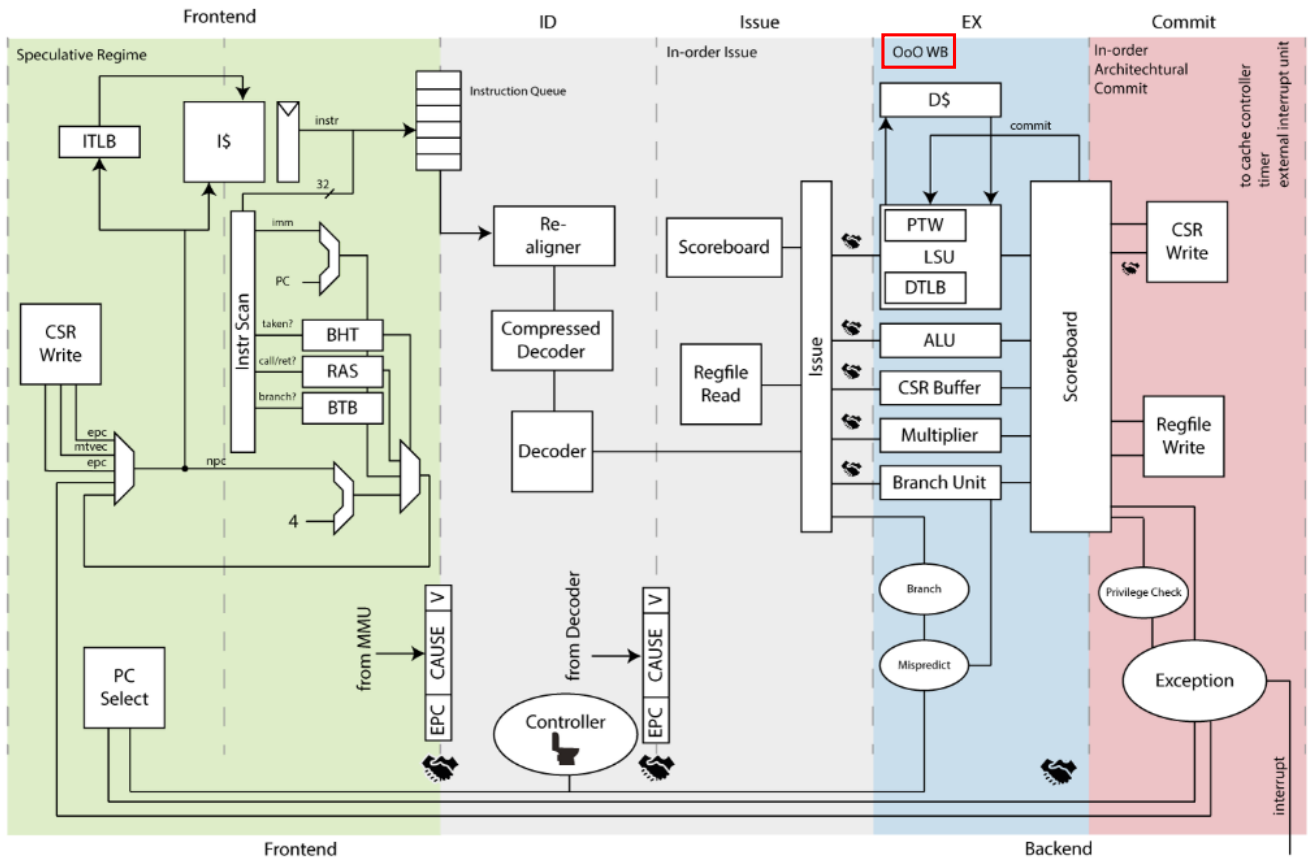
\includegraphics[width=0.75\linewidth]{images/cva6-simplified-overview.png}
    \caption{Overview of the 6-stage pipeline of CVA6}
    \label{fig:cva6-pipeline}
\end{figure}

In addition to the cache memory, the CVA6 processor contains 2 Register File units, one for reading present on the issue stage of the pipeline and one for writing located in the commit stage. These units will be crucial components to alter and adapt for the implementation of the streaming engine.

The flow of this pipeline starts in the frontend section where the \acrfull{PC} is updated according to the execution signals. These signals can indicate a normal advance across the executing process instructions or a modification according to branch prediction information, exceptions, or pipeline flushes. The instructions are then translated from the \acrshort{PC} in the instruction fetch section of the frontend, and stored on the instruction queue. In the instruction decoding stage, an instruction is taken from the queue. It realigns, decompresses, and decodes the instruction, passing it to the issue stage, where it will await the availability of its operands. Execution is made out-of-order in the execution stage, which is possible thanks to the \acrfull{ROB} and scoreboard in the commit stage. This last stage uses the information stored in the \acrshort{ROB} in order to commit the instructions in the order in which they were issued, and the register files and data held in the cache are written to memory.


Studies conducted by Zaruba and Luca Benini \cite{8777130} using a hardware implementation of the CVA6 processor, revealed that using instructions extensions like SIMD on the CVA6 architecture improves its power em efficiency when comparing it to a base-line implementation of the processor running at higher frequencies. This can indicate that the features proposed with UVE and streaming support will most likely bring gains to the CVA6 overall performance.


The expandable nature and simple design of this 6-stage CPU make it the perfect candidate for the implementation of the proposed streaming engine on a hardware description, enhancing its capabilities without much complexity added to the design.

%the cache subsystem includes the data miss unit, the data controller, and the data buffer. These functional units play a crucial role in ensuring the seamless execution of processes related to data fetching, storing, and buffering of the instruction and data memory caches.



\subsection{Environment Setup and Preliminary Work}

Prior to starting the implementation of the Unlimited Vector Extension (UVE) and streaming engine in the CVA6 CPU architecture, the initial step involved configuring a working environment.

In order to adapt the original CVA6 architecture to support the Unlimited Vector Extension (UVE) and to integrate a streaming engine in the CVA6 CPU architecture, a Linux environment had to be configured with the correct set of tools.  This task was undertaken during the initial stages of the 2nd Cycle Integrated Project in Electrical and Computer Engineering. It encompassed the setup of the following tools:
\begin{itemize}
    \item \textbf{Verilator}\cite{Verilator, Verilator-Doc}: A System Verilog simulator used for testing the CPU description and conducting simulations of the described hardware.
    \item \textbf{RISC-V Toolchain}\cite{RV-Doc}: The ISA  binarys utilized, for compiling the CVA6 RISC-V source code.
    \item \textbf{RISC-V Proxy Kernel}\cite{RV-PK}: The RISC-V compiled engine executed using the Verilator simulator for the CVA6.
    \item \textbf{Spike}\cite{Spike}: The RISC-V simulator employed for running RISC-V compiled applications.
\end{itemize}


Setting up this environment turned out to be more intricate than initially anticipated. After a successful installation and configuration of all the tools were achieved, some simple modifications and tests were made to the CVA6 architecture and the RISC-V \acrshort{ISA} to validate that the configuration of the environment was correct,.

These modifications included introducing a set of new custom instructions in the RISC-V ISA and modifying the CVA6 CPU architecture to integrate these instructions into the decoding unit of the CPU. This extension enabled the decoding unit to process the new instructions and appropriately dispatch operations to the execution stage of the processor. Additionally, new functional units were implemented to effectively handle the operations associated with these custom instructions.

This initial work served as a simplified precursor to the more extensive developments that will be undertaken throughout the course of this thesis, like the implementation of the UVE ISA and the streaming engine.

\section{Proposed Architeture}

The implementation of the streaming engine on the CVA6 processor is likely to undergo several evolutions throughout the course of this thesis. Nevertheless this section presents the initial diagram for the implementation of the engine. This implementation is based on the one outlined in the Unlimited Vector Extension with Data Streaming Support paper \cite{uve-paper}. 
It involves modifying the decode, register file, and execution units to support not only the UVE instruction-set extension but also the support for vector processing including the vector registers and vector operations. The proposed register file modification can be resumed to adding a new set of stream registers, both in the read register file and the write register file. Additionally, it will also involve modifying the rename stage, which needs to be altered to support the renaming of vector registers and streams, and the commit stage to allow the commit and squash of streams in the streaming engine.

In addition to the modifications to the CPU architecture mentioned above, the implementation of the streaming engine itself is required. The placement of the streaming engine in the pipeline can be observed in Fig. \ref{fig:cva6-altered-pipeline}.
\begin{figure}[H]
    \centering
    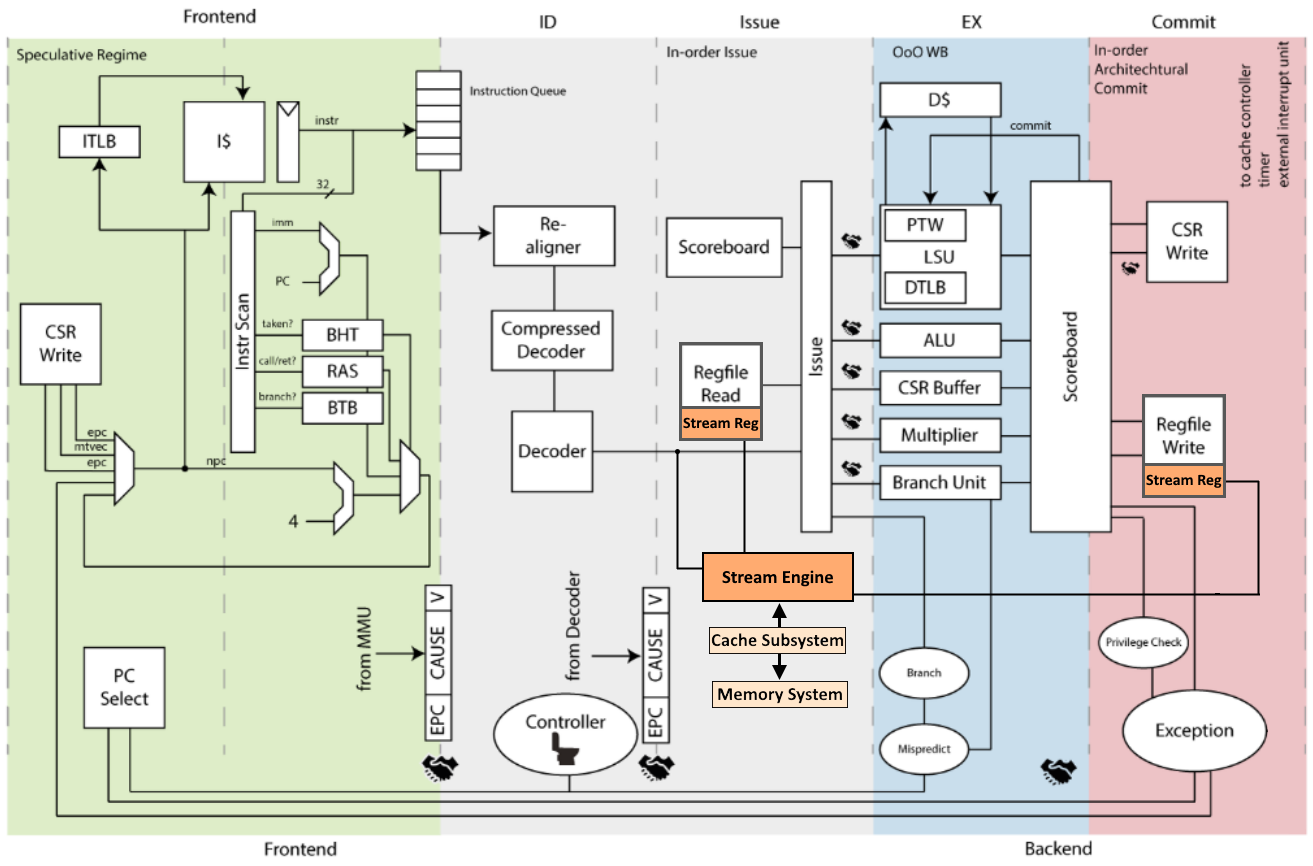
\includegraphics[width=0.75\linewidth]{images/cva6-overview-altered-simplified.png}
    \caption{CVA6 pipeline with Streaming Engine implementation}
    \label{fig:cva6-altered-pipeline}
\end{figure}


The initial proposal for the placement of the streaming engine is in the issue stage of the pipeline. The streaming engine will be directly connected to the newly integrated stream registers of the Read Register File and the Write Register File. 

It will also interface with the cache system however, some testing needs to be done in order to assess the best configuration. Connecting the stream engine to the L1 Cache could be simpler however, this level might have too much access stress, meaning that connecting to it could lead to a slowdown in memory access. Interfacing directly with L2 will not have the same stress problem as L1 but can lead to a memory incoherence problem,  for this reason, a well-thought-out choice will need to be made.

Besides connecting to the cache subsystems, the streaming engine will also be connected directly to the system's memory, allowing it to perform memory requests through its memory request queue.


The design and internal architecture of the streaming engine to be implemented on the CVA6 processor will be based on the one proposed by Xavier Fernandes in his thesis entitled "Data-Streaming Engine Architecture for the Unlimited Vector Extension" \cite{thesis-xf}. The original engine's internal architecture can be seen in the diagram in Fig. \ref{fig:xav-engine}.

\begin{figure}[H]
    \centering
    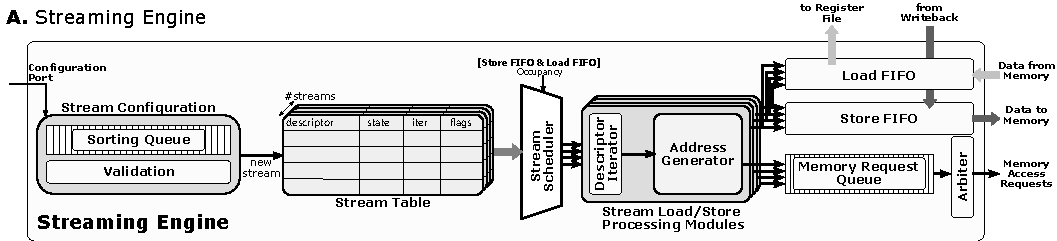
\includegraphics[width=1\linewidth]{images/uve-engine.pdf}
    \caption{Streaming Engine Inner Architeture}
    \label{fig:xav-engine}
\end{figure}

The engine proposed by Xavier Fernandes \cite{thesis-xf} maintains a similar structure to the original streaming engine however, the developed implementation was designed using 5 interconnected modules:
\begin{itemize}
    \item The \textbf{Stream Configuration} module, responsible for the configuration of the streams to be utilized by the engine;
    \item The \textbf{Stream State} module, which corresponds to the stream table unit, the stream scheduler, and the address generator part of the originally proposed streaming engine, is the central part of the streaming engine entrusted with keeping the record of each stream and generating the corresponding memory addresses.
    \item The \textbf{Stream Iterator}, a module closely coupled with the Stream State module and used to advance the configured stream descriptors and update the stored stream states.
    \item The \textbf{Load Memory Management Unit (MMU)} comprises a FIFO unit and the memory request queue. This module is responsible for managing the memory requests that need to be made and provide the corresponding data back to the processing units.
    \item The \textbf{Store Memory Management Unit (MMU)} stores the memory addresses corresponding to the active stream configurations and awaits the arrival of data to be stored in memory.
    
\end{itemize}

The envisaged approach to implement this infrastructure will consider the adaptation of this streaming engine and its corresponding modules and signals to the architecture of the CVA6 processor, creating the first hardware description implementation of this system.


\section{Workload Tests and System Evaluation}
The UVE and streaming engine proposed by Domingos et al. \cite{uve-paper} have undergone evaluation and testing in the Gem5 simulator as a proof-of-concept. However, to date, no hardware implementation has been executed, and therefore, no testing in a hardware environment has taken place.

With the objective of this thesis being the development of a hardware configuration for the UVE and streaming engine, it will be possible to conduct tests and comparisons against other hardware implementations of vector extensions and streaming engine platforms.

The results extracted from the final implementation will encompass:
\begin{itemize}
    \item \textbf{Performance Evaluation}: Through a series of workload tests, the achieved performance gains will be assessed and compared to the baseline version of the CVA6.
    \item \textbf{Energy Consumption}: With a hardware description of the CVA6 processor, it will be possible to evaluate the energy consumed during the execution of the workload tests. Specifically, it will be analyzed the energy increase associated with the version implementing the streaming engine.
    \item \textbf{Design Footprint}: Similar to energy consumption, the hardware description of the streaming engine implemented in the CVA6 architecture will enable an analysis of the total increase in area resulting from the implementation of the streaming engine.
\end{itemize}

The final developed CPU hardware description can serve as the infrastructure for further research in regard to improvements in the UVE ISA as well as the streaming engine architecture. 

